% Options for packages loaded elsewhere
% Options for packages loaded elsewhere
\PassOptionsToPackage{unicode}{hyperref}
\PassOptionsToPackage{hyphens}{url}
\PassOptionsToPackage{dvipsnames,svgnames,x11names}{xcolor}
%
\documentclass[
  letterpaper,
  DIV=11,
  numbers=noendperiod]{scrreprt}
\usepackage{xcolor}
\usepackage{amsmath,amssymb}
\setcounter{secnumdepth}{5}
\usepackage{iftex}
\ifPDFTeX
  \usepackage[T1]{fontenc}
  \usepackage[utf8]{inputenc}
  \usepackage{textcomp} % provide euro and other symbols
\else % if luatex or xetex
  \usepackage{unicode-math} % this also loads fontspec
  \defaultfontfeatures{Scale=MatchLowercase}
  \defaultfontfeatures[\rmfamily]{Ligatures=TeX,Scale=1}
\fi
\usepackage{lmodern}
\ifPDFTeX\else
  % xetex/luatex font selection
\fi
% Use upquote if available, for straight quotes in verbatim environments
\IfFileExists{upquote.sty}{\usepackage{upquote}}{}
\IfFileExists{microtype.sty}{% use microtype if available
  \usepackage[]{microtype}
  \UseMicrotypeSet[protrusion]{basicmath} % disable protrusion for tt fonts
}{}
\makeatletter
\@ifundefined{KOMAClassName}{% if non-KOMA class
  \IfFileExists{parskip.sty}{%
    \usepackage{parskip}
  }{% else
    \setlength{\parindent}{0pt}
    \setlength{\parskip}{6pt plus 2pt minus 1pt}}
}{% if KOMA class
  \KOMAoptions{parskip=half}}
\makeatother
% Make \paragraph and \subparagraph free-standing
\makeatletter
\ifx\paragraph\undefined\else
  \let\oldparagraph\paragraph
  \renewcommand{\paragraph}{
    \@ifstar
      \xxxParagraphStar
      \xxxParagraphNoStar
  }
  \newcommand{\xxxParagraphStar}[1]{\oldparagraph*{#1}\mbox{}}
  \newcommand{\xxxParagraphNoStar}[1]{\oldparagraph{#1}\mbox{}}
\fi
\ifx\subparagraph\undefined\else
  \let\oldsubparagraph\subparagraph
  \renewcommand{\subparagraph}{
    \@ifstar
      \xxxSubParagraphStar
      \xxxSubParagraphNoStar
  }
  \newcommand{\xxxSubParagraphStar}[1]{\oldsubparagraph*{#1}\mbox{}}
  \newcommand{\xxxSubParagraphNoStar}[1]{\oldsubparagraph{#1}\mbox{}}
\fi
\makeatother

\usepackage{color}
\usepackage{fancyvrb}
\newcommand{\VerbBar}{|}
\newcommand{\VERB}{\Verb[commandchars=\\\{\}]}
\DefineVerbatimEnvironment{Highlighting}{Verbatim}{commandchars=\\\{\}}
% Add ',fontsize=\small' for more characters per line
\usepackage{framed}
\definecolor{shadecolor}{RGB}{241,243,245}
\newenvironment{Shaded}{\begin{snugshade}}{\end{snugshade}}
\newcommand{\AlertTok}[1]{\textcolor[rgb]{0.68,0.00,0.00}{#1}}
\newcommand{\AnnotationTok}[1]{\textcolor[rgb]{0.37,0.37,0.37}{#1}}
\newcommand{\AttributeTok}[1]{\textcolor[rgb]{0.40,0.45,0.13}{#1}}
\newcommand{\BaseNTok}[1]{\textcolor[rgb]{0.68,0.00,0.00}{#1}}
\newcommand{\BuiltInTok}[1]{\textcolor[rgb]{0.00,0.23,0.31}{#1}}
\newcommand{\CharTok}[1]{\textcolor[rgb]{0.13,0.47,0.30}{#1}}
\newcommand{\CommentTok}[1]{\textcolor[rgb]{0.37,0.37,0.37}{#1}}
\newcommand{\CommentVarTok}[1]{\textcolor[rgb]{0.37,0.37,0.37}{\textit{#1}}}
\newcommand{\ConstantTok}[1]{\textcolor[rgb]{0.56,0.35,0.01}{#1}}
\newcommand{\ControlFlowTok}[1]{\textcolor[rgb]{0.00,0.23,0.31}{\textbf{#1}}}
\newcommand{\DataTypeTok}[1]{\textcolor[rgb]{0.68,0.00,0.00}{#1}}
\newcommand{\DecValTok}[1]{\textcolor[rgb]{0.68,0.00,0.00}{#1}}
\newcommand{\DocumentationTok}[1]{\textcolor[rgb]{0.37,0.37,0.37}{\textit{#1}}}
\newcommand{\ErrorTok}[1]{\textcolor[rgb]{0.68,0.00,0.00}{#1}}
\newcommand{\ExtensionTok}[1]{\textcolor[rgb]{0.00,0.23,0.31}{#1}}
\newcommand{\FloatTok}[1]{\textcolor[rgb]{0.68,0.00,0.00}{#1}}
\newcommand{\FunctionTok}[1]{\textcolor[rgb]{0.28,0.35,0.67}{#1}}
\newcommand{\ImportTok}[1]{\textcolor[rgb]{0.00,0.46,0.62}{#1}}
\newcommand{\InformationTok}[1]{\textcolor[rgb]{0.37,0.37,0.37}{#1}}
\newcommand{\KeywordTok}[1]{\textcolor[rgb]{0.00,0.23,0.31}{\textbf{#1}}}
\newcommand{\NormalTok}[1]{\textcolor[rgb]{0.00,0.23,0.31}{#1}}
\newcommand{\OperatorTok}[1]{\textcolor[rgb]{0.37,0.37,0.37}{#1}}
\newcommand{\OtherTok}[1]{\textcolor[rgb]{0.00,0.23,0.31}{#1}}
\newcommand{\PreprocessorTok}[1]{\textcolor[rgb]{0.68,0.00,0.00}{#1}}
\newcommand{\RegionMarkerTok}[1]{\textcolor[rgb]{0.00,0.23,0.31}{#1}}
\newcommand{\SpecialCharTok}[1]{\textcolor[rgb]{0.37,0.37,0.37}{#1}}
\newcommand{\SpecialStringTok}[1]{\textcolor[rgb]{0.13,0.47,0.30}{#1}}
\newcommand{\StringTok}[1]{\textcolor[rgb]{0.13,0.47,0.30}{#1}}
\newcommand{\VariableTok}[1]{\textcolor[rgb]{0.07,0.07,0.07}{#1}}
\newcommand{\VerbatimStringTok}[1]{\textcolor[rgb]{0.13,0.47,0.30}{#1}}
\newcommand{\WarningTok}[1]{\textcolor[rgb]{0.37,0.37,0.37}{\textit{#1}}}

\usepackage{longtable,booktabs,array}
\usepackage{calc} % for calculating minipage widths
% Correct order of tables after \paragraph or \subparagraph
\usepackage{etoolbox}
\makeatletter
\patchcmd\longtable{\par}{\if@noskipsec\mbox{}\fi\par}{}{}
\makeatother
% Allow footnotes in longtable head/foot
\IfFileExists{footnotehyper.sty}{\usepackage{footnotehyper}}{\usepackage{footnote}}
\makesavenoteenv{longtable}
\usepackage{graphicx}
\makeatletter
\newsavebox\pandoc@box
\newcommand*\pandocbounded[1]{% scales image to fit in text height/width
  \sbox\pandoc@box{#1}%
  \Gscale@div\@tempa{\textheight}{\dimexpr\ht\pandoc@box+\dp\pandoc@box\relax}%
  \Gscale@div\@tempb{\linewidth}{\wd\pandoc@box}%
  \ifdim\@tempb\p@<\@tempa\p@\let\@tempa\@tempb\fi% select the smaller of both
  \ifdim\@tempa\p@<\p@\scalebox{\@tempa}{\usebox\pandoc@box}%
  \else\usebox{\pandoc@box}%
  \fi%
}
% Set default figure placement to htbp
\def\fps@figure{htbp}
\makeatother





\setlength{\emergencystretch}{3em} % prevent overfull lines

\providecommand{\tightlist}{%
  \setlength{\itemsep}{0pt}\setlength{\parskip}{0pt}}



 


\KOMAoption{captions}{tableheading}
\makeatletter
\@ifpackageloaded{tcolorbox}{}{\usepackage[skins,breakable]{tcolorbox}}
\@ifpackageloaded{fontawesome5}{}{\usepackage{fontawesome5}}
\definecolor{quarto-callout-color}{HTML}{909090}
\definecolor{quarto-callout-note-color}{HTML}{0758E5}
\definecolor{quarto-callout-important-color}{HTML}{CC1914}
\definecolor{quarto-callout-warning-color}{HTML}{EB9113}
\definecolor{quarto-callout-tip-color}{HTML}{00A047}
\definecolor{quarto-callout-caution-color}{HTML}{FC5300}
\definecolor{quarto-callout-color-frame}{HTML}{acacac}
\definecolor{quarto-callout-note-color-frame}{HTML}{4582ec}
\definecolor{quarto-callout-important-color-frame}{HTML}{d9534f}
\definecolor{quarto-callout-warning-color-frame}{HTML}{f0ad4e}
\definecolor{quarto-callout-tip-color-frame}{HTML}{02b875}
\definecolor{quarto-callout-caution-color-frame}{HTML}{fd7e14}
\makeatother
\makeatletter
\@ifpackageloaded{bookmark}{}{\usepackage{bookmark}}
\makeatother
\makeatletter
\@ifpackageloaded{caption}{}{\usepackage{caption}}
\AtBeginDocument{%
\ifdefined\contentsname
  \renewcommand*\contentsname{Table of contents}
\else
  \newcommand\contentsname{Table of contents}
\fi
\ifdefined\listfigurename
  \renewcommand*\listfigurename{List of Figures}
\else
  \newcommand\listfigurename{List of Figures}
\fi
\ifdefined\listtablename
  \renewcommand*\listtablename{List of Tables}
\else
  \newcommand\listtablename{List of Tables}
\fi
\ifdefined\figurename
  \renewcommand*\figurename{Figure}
\else
  \newcommand\figurename{Figure}
\fi
\ifdefined\tablename
  \renewcommand*\tablename{Table}
\else
  \newcommand\tablename{Table}
\fi
}
\@ifpackageloaded{float}{}{\usepackage{float}}
\floatstyle{ruled}
\@ifundefined{c@chapter}{\newfloat{codelisting}{h}{lop}}{\newfloat{codelisting}{h}{lop}[chapter]}
\floatname{codelisting}{Listing}
\newcommand*\listoflistings{\listof{codelisting}{List of Listings}}
\makeatother
\makeatletter
\makeatother
\makeatletter
\@ifpackageloaded{caption}{}{\usepackage{caption}}
\@ifpackageloaded{subcaption}{}{\usepackage{subcaption}}
\makeatother
\usepackage{bookmark}
\IfFileExists{xurl.sty}{\usepackage{xurl}}{} % add URL line breaks if available
\urlstyle{same}
\hypersetup{
  pdftitle={Data},
  pdfauthor={FURao},
  colorlinks=true,
  linkcolor={blue},
  filecolor={Maroon},
  citecolor={Blue},
  urlcolor={Blue},
  pdfcreator={LaTeX via pandoc}}


\title{Data}
\author{FURao}
\date{2025-08-05}
\begin{document}
\maketitle

\renewcommand*\contentsname{Table of contents}
{
\hypersetup{linkcolor=}
\setcounter{tocdepth}{2}
\tableofcontents
}

\bookmarksetup{startatroot}

\chapter*{前言}\label{ux524dux8a00}
\addcontentsline{toc}{chapter}{前言}

\markboth{前言}{前言}

数据学习过程中的笔记,希望能够对大家也有所帮助。

\bookmarksetup{startatroot}

\chapter{简介}\label{ux7b80ux4ecb}

学习数据分析过程的笔记。

\bookmarksetup{startatroot}

\chapter{Summary}\label{summary}

In summary, this book has no content whatsoever.

\begin{Shaded}
\begin{Highlighting}[]
\DecValTok{1} \SpecialCharTok{+} \DecValTok{1}
\end{Highlighting}
\end{Shaded}

\begin{verbatim}
[1] 2
\end{verbatim}

\bookmarksetup{startatroot}

\chapter{行业指标梳理}\label{ux884cux4e1aux6307ux6807ux68b3ux7406}

\section{概览}\label{ux6982ux89c8}

  本章是\textbf{行业的指标梳理}。主要分为电商(E-commerce)、短视频(Short
Video)、直播/直播电商(Live)、社交媒体(Social Media)、风控。

  指标体系的\textbf{目的}是为了了解业务全貌,快速业务定位问题、以及明确解决方案。

  \textbf{首先},是要确定我们的战略目标,以及与之对应的北极星指标。\textbf{第二步},看为了达到这个北极星指标所需要达到业务链路是哪些(例如AARRR模型:Acquistion:获取用户;Activation:提高活跃度;Retention:提高留存率;Revenue:获取收入;Refer:自传播)。\textbf{第三步},围绕业务流程设计维度和指标。\textbf{第四步},最后用趋势、对比、细分、分布的方式去aggregate各种指标;{趋势}即通过折线图看到数据指标的走势和波动,让涨跌幅度可视化;{对比}包括同比和环比,同比是指今年某月/某季度和去年某月/某季度相比,环比可以是环比上周/上月;对比数据除了能反映出业务发展情况之外,还可以帮助排除季节性或周期性的影响因素;{细分}是指某个指标的具体来源组成,比如在看商品详情页的曝光量的时候,不仅要看总曝光量,还要分析每个曝光是从哪个页面进来的(首页、活动页、搜索框、商品分类页、排行榜页等等);{分布}是指某个指标的来源占比,比如上面这个商品的曝光量来源。\textbf{第五步},形成分析SOP和数据看板。

  

\section{电子商务(Ecommerce)}\label{ux7535ux5b50ux5546ux52a1ecommerce}

  并非所有的指标都有价值,我们需要确定需要跟踪的关键绩效指标(KPI)来提高绩效。在线销售是可靠增长是来自于分析业务不同部分随时间变化的绩效。随着时sss间的推移,跟踪正确是指标将提高在线销售。行业有着共同的KPI,但是每个企业都有独特的KPI需要定期跟踪和分析,以改进其产品、服务或与客户的互动。All
KPIs are metrics;not all metrics are KPIs.

\subsection{Mindmap}\label{mindmap}

\includegraphics[width=6.1in,height=2.52in]{01metrics_files/figure-latex/mermaid-figure-1.png}

\includegraphics[width=8.04in,height=5.36in]{01metrics_files/figure-latex/mermaid-figure-24.png}

\includegraphics[width=9.55in,height=3.05in]{01metrics_files/figure-latex/mermaid-figure-23.png}

\includegraphics[width=8.12in,height=3.57in]{01metrics_files/figure-latex/mermaid-figure-22.png}

  其中RFM分类如下表所示,可以基于此给用户打分。

\begin{longtable}[]{@{}
  >{\raggedright\arraybackslash}p{(\linewidth - 6\tabcolsep) * \real{0.2500}}
  >{\raggedright\arraybackslash}p{(\linewidth - 6\tabcolsep) * \real{0.3611}}
  >{\raggedright\arraybackslash}p{(\linewidth - 6\tabcolsep) * \real{0.1944}}
  >{\raggedright\arraybackslash}p{(\linewidth - 6\tabcolsep) * \real{0.1944}}@{}}
\toprule\noalign{}
\begin{minipage}[b]{\linewidth}\raggedright
用户分类
\end{minipage} & \begin{minipage}[b]{\linewidth}\raggedright
最近一次消费时间间隔 (R)
\end{minipage} & \begin{minipage}[b]{\linewidth}\raggedright
消费频率 (F)
\end{minipage} & \begin{minipage}[b]{\linewidth}\raggedright
消费金额 (M)
\end{minipage} \\
\midrule\noalign{}
\endhead
\bottomrule\noalign{}
\endlastfoot
1. 重要价值用户 & 高 & 高 & 高 \\
2. 重要发展用户 & 高 & 低 & 高 \\
3. 重要保持用户 & 低 & 高 & 高 \\
4. 重要挽留用户 & 低 & 低 & 高 \\
5. 一般价值用户 & 高 & 高 & 低 \\
6. 一般发展用户 & 高 & 低 & 低 \\
7. 一般保持用户 & 低 & 高 & 低 \\
8. 一般挽留用户 & 低 & 低 & 低 \\
\end{longtable}

  AARRR分类如下图所示:

\includegraphics[width=5.75in,height=9.04in]{01metrics_files/figure-latex/mermaid-figure-21.png}

\begin{itemize}
\item
  \textbf{K-factor}是用来衡量\textbf{产品病毒式传播能力}的指标。它告诉我们平均每个现有的用户能够带来多少新用户。

  \begin{itemize}
  \tightlist
  \item
    计算公式:(每个用户发送的邀请数)*(邀请的转化率)
  \item
    大于1意味着用户会自然增长,因为每个用户带来的新用户不止一个。这通常是产品获得病毒式增长的标志;小于1意味着产品需要通过其他营销手段来获取新用户。
  \end{itemize}
\item
  \textbf{NPS(Net Promoter
  Score)}是衡量\textbf{客户忠诚度}和\textbf{推荐意愿}的指标。

  \begin{itemize}
  \item
    通过询问客户``有多大程度上愿意向朋友或者同事推荐产品''来衡量。根据得分,用户被分为三类:

    \begin{itemize}
    \item
      推荐者(Promoters):9-10分,是忠实且热情的用户
    \item
      被动者(Passives):7-8分,对产品满意但不热情,容易被竞争对手吸引
    \item
      贬损者(Detractors):0-6,对产品不满,可能传播负面口碑
    \end{itemize}
  \item
    最终分数:NPS = (推荐者百分比)-(贬损者百分比)
  \end{itemize}
\end{itemize}

\includegraphics[width=13.99in,height=4.73in]{01metrics_files/figure-latex/mermaid-figure-20.png}

\includegraphics[width=10.64in,height=3.71in]{01metrics_files/figure-latex/mermaid-figure-19.png}

\includegraphics[width=9.21in,height=4.33in]{01metrics_files/figure-latex/mermaid-figure-18.png}

\subsection{关键电商指标}\label{ux5173ux952eux7535ux5546ux6307ux6807}

\subsubsection{\texorpdfstring{\textbf{电商销售方面指标}}{电商销售方面指标}}\label{ux7535ux5546ux9500ux552eux65b9ux9762ux6307ux6807}

  这些指标侧重于:运营和改进电子商务商店、在线销售和支付以及增加的收入。

\textbf{一、转化率}

  访问网站并查看产品后购买的客户数量。代表了基于客户查看产品
的实际销售额。将其与页面浏览量、平均订单价值和流量来源进行比较,可以更深入地了解用户行为。

\textbf{二、毛利率}

  实际利率。

\textbf{三、平均订单价值(AOV)}

  平均客户订单的货币价值。还需要跟踪平均放弃订单价值(AAOV),即在后买的结账或购物车阶段放弃的订单的平均价值。从整体上跟踪AOV,然后按设备类型、平台、流量来源进行细分。确定AOV最高的客户来源可以帮助我们开展更多高投资回报率的营销活动。

\textbf{四、每次获取成本}

  获得新用户的成本。包括广告成本、电子邮件活动、提供的折扣以及实际向客户进行销售所需的任何其他费用。可以了解真正获得付费客户需要付出的成本。可以与许多其他指标进行比较,包括平均订单价值、流量、客户生命周期价值等等,以了解赢得客户的成本。

\textbf{五、购物车放弃率}

  指将商品添加购物车后放弃购买的客户百分比。添加到购物车的商品数量、添加到购物车的商品价值以及他们购物的时间也都很重要。通过跟踪此指标,可以深入了解有多少客户对产品感兴趣但是没有继续购买。通过将其与此列表中的其他指标进行比较,可以制定降低放弃率并吸引更多客户进行销售的营销方案。

\textbf{六、结账放弃率}

  启动结账然后放弃购买的客户的百分比。这比购物车放弃更近一步,这以为这我们花费了更多的精力来让他们达到那个阶段。跟踪这个指标为我们提供了有关客户准备购买后未完成交易的具体信息。

\textbf{七、客户终身价值(复购)}

  客户终身价值(CLV)是作为用户的每个人的整个生命周期中平均赚取的收入金额。它本质上分解了一个客户对于我们来说的平均价值,并区分了现在购买200元的客户好在未来五年内购买100元产品10次的客户-----哪一个实际上对我们更有价值。这个指标使得我们深入了解每个客户对我们的价值。将其直接与客户获取成本、转化率、流量进行比较,以了解营销和客户获取活动的投资回报率。

\textbf{八、广告支出收入}

  将收入除广告成本,可以获得基于广告成本的平均回报收入的比率,该值是我们从每笔广告费中赚取的金额。跟踪它,使得我们根据当前成本和收入衡量赚取收入的平均广告成本。我们可以使用它来深入了解让客户完成购买需要花费多少广告费用。我们致力于通过尝试新的、更有效的广告方法来提高广告的投资回报率。

\subsubsection{\texorpdfstring{\textbf{用户体验方面指标}}{用户体验方面指标}}\label{ux7528ux6237ux4f53ux9a8cux65b9ux9762ux6307ux6807}

  这些指标侧重于:用户如何使用我们的产品并与之互动、服务性能和速度、跨设备类型和平台的完善服务以及网站流量。

\textbf{九、设备类型}

  按照设备类型细分,以进一步了解哪些设备更频繁地使用,并针对每种设备类型定制网站的用户体验。跟踪这个指标可以为每个平台构建移动优化体验。尝试在不同设备类型之间保持一致的流程,但在不同设备(移动设备、网络和平板电脑)上测试性能,以了解客户的购买方式以及那种设备的工作效率最高。

\textbf{十、网站速度}

  网站速度和结账加载时间对于维护和吸引电子商务网站上的客户非常重要。电子商务平台的性能、效率和速度是购物者体验的核心。监控页面的速度,特别注意与购物车和结账相关的页面。

\textbf{十一、客户参与}

  客户对服务的参与程度,通常使用反应、分享和订阅来衡量。客户越活跃、越感兴趣,就越有可能购买、分享。我们可能需要跟踪的包括:用户在商店页面上停留的时间、用户最倾向点击每个页面的哪些区域、访问网站后再次访问的比率、通过社交渠道分享的用户、关注一些实时营销渠道并不取消订阅的用户等等。跟踪这个指标可以衡量用户在产品体验中的活跃程度和沉浸程度,因为这种活动和兴趣可以转化为忠诚度和收入。

\textbf{十二、跳出率}

  指仅访问一个页面后突然离开网站的客户比例。这通常说明存在着严重的用户体验问题,例如页面加载缓慢、外观或者导航延迟,也可能是营销定位不佳的迹象,因为广告所带来的客户没有在网站或待售产品中找到价值。我们使用跳出率来激励提高网站或应用程序的粘性。制定策略以降低跳出率,让更多的客户对产品感兴趣,建立客户忠诚度并引导购买。

\subsubsection{\texorpdfstring{\textbf{客户支持与满意度方面指标}}{客户支持与满意度方面指标}}\label{ux5ba2ux6237ux652fux6301ux4e0eux6ee1ux610fux5ea6ux65b9ux9762ux6307ux6807}

  这些指标侧重于:客户需要哪些支持方法、何时将用户连接到支持的最佳实践,以及捕获有关平台的有用反馈。

\textbf{十三、客户调查结果和反馈}

  定期进行客户调查并获得反馈,尤其在网站发生更改或者引入新功能时。愿意留下反馈的客户百分比是衡量客户对应用和产品感兴趣的一个指标。用户没有离开去并一个电子商务网站,而是给出反馈并希望得到改善。

\textbf{十四、客户评论}

  了解客户想法、需求。

\textbf{十五、客户联系方式(电话、邮箱)}

  注意用户最常使用的渠道。

\textbf{十六、平均工单解决时间}

  也成为服务级别协议时间(SLA)。跟踪平均SLA以及从工单创建到解决(打开到关闭)的平均时间。缩短平均响应时间意味着首次购物者将有可能重复购买。

\subsubsection{\texorpdfstring{\textbf{营销方面指标}}{营销方面指标}}\label{ux8425ux9500ux65b9ux9762ux6307ux6807}

  这些指标侧重于:网站流量、客户参与方法和曝光度。

\textbf{十七、流量来源}

  确定顾客来源的主要渠道,以帮助改进营销和广告。来源包括付费广告、自然搜索网站、推荐、直接输入网页等等。分析以利用最佳渠道。加倍关注被证明有效的流量来源,并减少对流量产生最低的来源的工作量。

\textbf{十八、流量}

  以用户以及用户访问时间来衡量。可以作为一个整体来研究,也可以细分为更具体的一些指标,例如每次访问的页面的浏览量、网站停留时间、跳出率、新客户和回头客。衡量流量峰值以及平均值,并将这些数据与电商销售指标结合,以得出有关转化率、放弃和投资回报率的观点。

\textbf{十九、社媒参与度(关注、参与、分享)和浏览量}

  提供直接的沟通渠道。利用这种交流与客户建立关系,从而培养未来的忠诚用户;并帮助制定的社交媒体策略,提升影响力。进一步,虽然病毒式的传播可能具有价值,但是建立稳定。忠诚的读者群是建立可持续增长和可靠收入来源的更好方法。

\subsection{如何选择KPI}\label{ux5982ux4f55ux9009ux62e9kpi}

  使用\textbf{SMART}方法。

\subsubsection{S.Specific}\label{s.specific}

  KPI必须清晰、明确,不能模糊不清。不能是模糊的``提高销售额'',而应该说``将本季度的线上销售额提高10\%''。

\subsubsection{M.Measurable}\label{m.measurable}

  必须是可以量化,可以被追踪、衡量的。比如``新增500个用户''。

\subsubsection{A.Achievable}\label{a.achievable}

  必须显示可达成,不可假大空。

\subsubsection{R.Relevant}\label{r.relevant}

  与现实业务关联。

\subsubsection{T.Time-bound}\label{t.time-bound}

  必须有明确的截止日期。

\section{短视频Short Video}\label{ux77edux89c6ux9891short-video}

\subsection{短视频平台的生产机制}\label{ux77edux89c6ux9891ux5e73ux53f0ux7684ux751fux4ea7ux673aux5236}

  短视频平台用算法和激励制造出流量繁荣的假象,但背后创作者、用户和生态本身都在被慢慢消耗,这种机制既让平台看起来很繁荣,但是暗中积累``内伤''。如下图所示:

\includegraphics[width=6.47in,height=11.46in]{01metrics_files/figure-latex/mermaid-figure-17.png}

\begin{itemize}
\item
  平台的算法分发决定了创作者的生存空间
\item
  创作者为了流量、收益等等不断生产内容
\item
  算法让大家卷到内容越来越同质化,最终影响创作生态
\end{itemize}

\subsection{内容创作}\label{ux5185ux5bb9ux521bux4f5c}

\begin{itemize}
\tightlist
\item
  \textbf{UGC}(User-Generated
  Content,用户生成内容),它指的是由品牌官方、专业机构、行业专家或拥有专业技能的创作者所制作的内容。主要形式包括:

  \begin{itemize}
  \item
    \textbf{原创短视频}:这是最基本的形式。用户通过拍摄、剪辑和配乐,创造出各种类型的原创内容,如日常生活分享、才艺展示、知识科普等。
  \item
    \textbf{挑战与热点话题}:平台会发起或用户自发形成各种挑战(Challenge)和热点话题,用户通过使用特定的
    BGM、滤镜或模板来参与,这会产生大量的 UGC 并形成病毒式传播。
  \item
    \textbf{合拍与二次创作}:用户可以通过``合拍''、``Stitch''等功能,对其他用户的视频进行再创作。这种互动模式鼓励了用户之间的交流,并不断产生新的内容。
  \item
    \textbf{评论与弹幕}:用户在视频下方的评论和弹幕,也属于 UGC
    的一种。它们是用户与内容互动、表达观点的直接方式,有助于形成社区氛围。
  \end{itemize}
\end{itemize}

  在短视频平台,UGC不仅仅是内容的来源,更是一种社交货币和用户参与感的体现。正是因为人人都可以成为创作者,才使得这类平台能够迅速积累海量内容和用户。

\begin{itemize}
\tightlist
\item
  \textbf{PGC}( \textbf{Professional-Generated Content}
  ,专业生成内容),它指的是由品牌官方、专业机构、行业专家或拥有专业技能的创作者所制作的内容。PGC通常具有较高的制作水准、更严谨的知识性或更强的权威性。
\item
  \textbf{OGC}( \textbf{Occupationally-generated Content}
  ,职业生成内容),这个概念用来描述介于 UGC(用户生成内容)和
  PGC(专业生成内容)之间的一种内容形态。

  \begin{itemize}
  \item
    \textbf{生产者}:OGC 的创作者通常是\textbf{独立的专业人士、行业 KOL
    (意见领袖)、或签约的媒体内容创作者}。他们依靠内容创作作为职业,具有一定的专业知识和制作能力。
  \item
    \textbf{特点}:OGC 往往拥有比 UGC 更高的制作水准和专业性,但又比 PGC
    更加独立和中立,不完全代表品牌官方的立场。
  \item
    \textbf{作用}:OGC
    在内容营销中扮演着重要的角色,它能以更客观、更具影响力的视角来传递信息,往往能获得消费者的信任。
  \item
    \textbf{举例}:品牌邀请一位头部博主拍摄的付费测评视频;一位专业的游戏主播制作的游戏攻略视频;一个独立的影评人撰写的影评文章。
  \end{itemize}
\end{itemize}

\pandocbounded{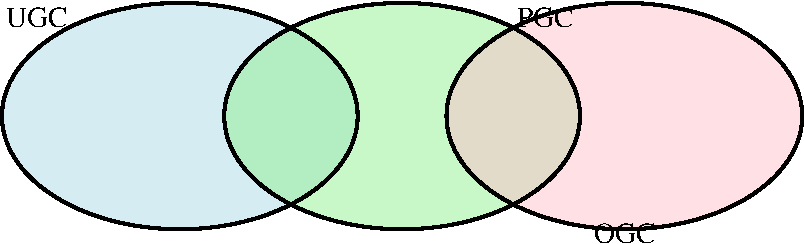
\includegraphics[keepaspectratio]{01metrics_files/figure-pdf/unnamed-chunk-10-1.pdf}}

\begin{itemize}
\item
  \textbf{UGC和PGC的区别}在于\textbf{有无专业的学识、资质},PGC的生产创作主体在所共享内容的领域具有一定的知识背景和工作资历,UGC则没有。
\item
  \textbf{PGC和OGC的区别}在于\textbf{是否领取相应报酬,}PGC的生产创作主体往往是出于``爱好'',义务的贡献内容,不收取报酬;而OGC是以职业为前提,其创作内容属于职务行为,获取报酬。
\item
  \textbf{UGC和OGC没有交集},在一个平台(网站)上,用户和提供商总是相对的,既是该平台的用户也是该平台的提供商的角色可能有,但属于极少的群体。
\item
  \textbf{PUGC(Professional User Generated
  Content},专业用户生产内容\textbf{)},以UGC形式产出的相对接近PGC的专业内容。PUGC模式是UGC、PGC模式发展中逐渐演化出的一种全新生产模式,率先由国内数字音频领域提出,后延伸到视频内容生产领域,被认为是``互联网短视频长远发展的趋势''。

  \begin{itemize}
  \item
    PUGC短视频既满足了用户对专业化、高品质内容的需求,又达到了贴近性且个性化的效果,满足了短视频用户的多种需求,极大程度提升了短视频平台内容的品味。
  \item
    YouTube与B站目前是全球PUGC较为集中的社交型视内容网站,其中B站已经在内容战略上明确转向``建设\textbf{PUGV(
    Professional User Generated Video)}社区''。
  \end{itemize}
\item
  \textbf{PUGC与PGC、UGC的关系}

  \begin{itemize}
  \item
    \textbf{从发展阶段上来说,PUGC是UGC、PGC模式在深度发育后为规避各自发展瓶颈而协商整合的结果。}

    \begin{itemize}
    \item
      PGC导向的长视颏(爱优腾)与UGC导向的短视频的平行发展格局已经确立,但两种生产方式的固有\textbf{弊病}也在逐渐极化:\textbf{UGC}尽管建构出生产的民主性与圈层化,但非专业性制作和扁平叙事造成了视觉品相的降低和叙事深度的缺失;\textbf{PGC}的专业研创保证了视觉与内容品质,但作为融媒体时代重要标志的个性化需求却被抑制。
    \item
      因而,业务界开始\textbf{寻求两种模式的组合}:专业用户生产内容(PUCC)由此产生。这种模式要求保留内容作者的个性,同时对内容生产全流程的专业性进行把控,不仅维系了内容作者的核心性,同时在其生产链中植入了``专业化''的模块。
    \end{itemize}
  \item
    \textbf{从生产模式来看,PUGC的生产链已经与传统UGC、PGC逐渐分异。}目前,以B站为代表的PUGC视频生产模式的主流策略基本采用几种方式:

    \begin{itemize}
    \item
      \textbf{以UP主本人为核心的视频内容}:利用专业团队辅助内容生产,以内容作者共同体的身份参与平台发布流程
    \item
      \textbf{专业视频内容团队直接生产内容,以作者身份在平台发布}
    \item
      \textbf{UP主本人通过平台专业技能培训计划或自行学习,生产专业内容在平台发布}
    \end{itemize}
  \item
    由此可见,PUGC的生产链已经与传统UGC、PGC逐渐分异:\textbf{内容作者仍位于生产链的中心位置,但``专业化模块''以各种形式介入生产流程。}这一独立的生产模式的形成对既有的UGC
    、PGC模式研究提出了新的要求,尤其对PUCC模式语境下的作者核心性和专业化方面的研究亟需展开。
  \end{itemize}
\item
  \textbf{MGC}(\textbf{Machine Generated
  Content,}机器生产内容或技术生产内容),指万物互联和全时在线的数据通过数据挖掘和智能算法生成海量的传感器资讯。如MGC新闻就是运用现代化的人工智能技术,由机器智能生产的新闻。通过摄像头、传感器、无人机等设备获取音视频线索,经由内部视频图像识别功能,让机器智能理解内容并做价值判断。随后与已有数据相关联,对语音语义进行检索和排列组合,智能生产审核新闻稿件,再经视频语音合成编辑、数据可视化系列过程,最终生成富媒体新闻。新华社发布的首条MGC视频新闻由媒体大脑中的``2410(智能媒体生产平台)''创造。
\end{itemize}

\subsection{生产消费}\label{ux751fux4ea7ux6d88ux8d39}

待补充

\subsection{Mindmap}\label{mindmap-1}

\includegraphics[width=4.83in,height=2.14in]{01metrics_files/figure-latex/mermaid-figure-16.png}

\includegraphics[width=10.92in,height=2.71in]{01metrics_files/figure-latex/mermaid-figure-15.png}

\includegraphics[width=10.3in,height=5.77in]{01metrics_files/figure-latex/mermaid-figure-14.png}

\includegraphics[width=10.79in,height=4.45in]{01metrics_files/figure-latex/mermaid-figure-13.png}

\includegraphics[width=9.69in,height=6.03in]{01metrics_files/figure-latex/mermaid-figure-12.png}

\section{直播Live}\label{ux76f4ux64adlive}

\includegraphics[width=2.77in,height=2.41in]{01metrics_files/figure-latex/mermaid-figure-11.png}

\includegraphics[width=8.56in,height=3.85in]{01metrics_files/figure-latex/mermaid-figure-10.png}

\includegraphics[width=9.77in,height=4.89in]{01metrics_files/figure-latex/mermaid-figure-9.png}

\includegraphics[width=9.88in,height=5.95in]{01metrics_files/figure-latex/mermaid-figure-8.png}

\section{社交媒体Social
Media}\label{ux793eux4ea4ux5a92ux4f53social-media}

\includegraphics[width=6.1in,height=4.31in]{01metrics_files/figure-latex/mermaid-figure-7.png}

\includegraphics[width=6.16in,height=4.06in]{01metrics_files/figure-latex/mermaid-figure-6.png}

\includegraphics[width=7.26in,height=4.96in]{01metrics_files/figure-latex/mermaid-figure-5.png}

\includegraphics[width=8.48in,height=4.28in]{01metrics_files/figure-latex/mermaid-figure-4.png}

\includegraphics[width=5.41in,height=3.79in]{01metrics_files/figure-latex/mermaid-figure-3.png}

\includegraphics[width=5.77in,height=2.57in]{01metrics_files/figure-latex/mermaid-figure-2.png}

\section{风控}\label{ux98ceux63a7}

\subsection{如何识别作弊用户}\label{ux5982ux4f55ux8bc6ux522bux4f5cux5f0aux7528ux6237}

  一般是爬虫或者渠道伪造的假用户

\begin{itemize}
\item
  分类问题可以用机器学习的分类算法

  \begin{itemize}
  \item
    渠道特征:渠道、渠道次日留存率、渠道流量、各种比率特征
  \item
    环境特征:设备(家用户以低端机为主)、系统(刷量的一般系统更新比较慢)、wifi使用情况、使用时间、来源地区、ip是否是
    blocked
  \item
    用户行为特征:访问时间、访问时长、访问页面、使用间隔、次日留存、活跃时间、页面跳转行为(假用户的行为要么多于一致,要么过于随机)、页面使用行为
  \item
    异常特征:设备号异常,ip异常(异地访问)、行为异常(突然大量点击广告、点赞)、数据包不完整
  \end{itemize}
\end{itemize}

\subsection{恶意刷单检测}\label{ux6076ux610fux5237ux5355ux68c0ux6d4b}

\begin{itemize}
\item
  机器学习分类算法

  \begin{itemize}
  \item
    商家特征:商家历史销量、信用、产品类别、发货快递公司等
  \item
    用户行为特征:用户信用、下单量、转化率、下单路径、浏览店铺行为、支付账号
  \item
    环境特征(主要是避免机器刷单):地区、ip、手机型号等
  \item
    异常检测:ip地址经常变动、经常清空cookie信息、账号近期交易成功率上升等
  \item
    评论文本检测:刷单的评论文本可能套路较为一致,计算与已标注评论文本的相似度作为特征
  \item
    图片相似度检测:同理,刷单可能重复利用图片进行评论
  \end{itemize}
\end{itemize}

\bookmarksetup{startatroot}

\chapter{ABTest}\label{abtest}

\section{概览}\label{ux6982ux89c8-1}

  本章介绍AB测试。\textbf{AB测试}(也称为随机对照试验 - RCT, Randomized
Controlled
Trial)是一种用于因果推断的实验设计方法。其核心在于通过\textbf{随机分配}将受试单元(用户、会话、页面访问等)分配到不同的处理组(通常是A:对照组/Baseline,B:新方案组),在控制其他变量(通过随机化)的前提下,比较不同处理对特定目标指标的影响,从而决定哪个更优。

  本章参考了@knuth84

\section{理论基础}\label{ux7406ux8bbaux57faux7840}

\subsection{因果推断的基石:潜在结果框架与随机化}\label{ux56e0ux679cux63a8ux65adux7684ux57faux77f3ux6f5cux5728ux7ed3ux679cux6846ux67b6ux4e0eux968fux673aux5316}

\begin{enumerate}
\def\labelenumi{\arabic{enumi}.}
\item
  \textbf{潜在结果框架(Neyman-Rubin Causal Model):}

  \begin{itemize}
  \item
    \textbf{定义}:对于每个实验单元\(i\)(用户、会话等),定义两个潜在结果:

    \begin{itemize}
    \item
      \(Y_i(1)\):单元\(i\)接受处理\(B\)(干预)时的结果
    \item
      \(Y_i(0)\):单元\(i\)接受处理\(A\)(对照)时的结果
    \end{itemize}
  \item
    \textbf{个体处理效应:}\(\text{ITE} = \tau_i = Y_i(1) - Y_i(0)\)
  \item
    \textbf{根本问题}:对于任何单元\(i\),我们只能观察到\(Y_i(1)\)或\(Y_i(0)\),永远无法同时观测两者,观察到的结果\(Y_i^{obs} = Z_i * Y_i(1) + (1 - Z_i) * Y_i(0)\),其中\(Z_i\)是指示变量,\(Z_i=1\)
    表示分配到\(B\)组,\(Z_i=0\) 表示分配到\(A\)组)。
  \item
    \textbf{目标}:估计\textbf{平均处理效应}\(\text{ATE} = \tau = E[\tau_i] = E[Y_i(1)-Y_i(0)]=E[Y(1)]-E[Y(0)]\)
  \end{itemize}
\item
  \textbf{随机化}
\end{enumerate}

\begin{itemize}
\item
  \textbf{关键假设(Ignorability/Unconfoundedness)}:通过\textbf{完全随机分配},我们确保处理分配\(Z_i\)独立于潜在结果,即\(Y_i(1),Y_i(0) \perp Z_i\),这意味着\(E[Y_i(1) | Z_i=1] = E[Y_i(1) | Z_i=0] = E[Y_i(1)]\)(同理于\(Y_i(0)\))。
\item
  \textbf{无偏估计量:}基于观测数据,ATE
  的一个简单无偏估计量是\textbf{组间均值差}\[\hat{τ}_{DiM} = \hat{E}[Y^{obs} | Z=1] - \hat{E}[Y^{obs} | Z=0] = \bar{Y}_B - \bar{Y}_A\]

  \begin{itemize}
  \item
    \textbf{证明无偏性}:
    \[E[\hat{τ}_{DiM}] = E[\bar{Y}_B - \bar{Y}_A] = E[\bar{Y}_B] - E[\bar{Y}_A] = E[Y(1) | Z=1] - E[Y(0) | Z=0]\](根据观测数据定义)

    由于随机化(\(Y_i(1),Y_i(0) \perp Z_i\)),有\(E[Y(1) | Z=1] = E[Y(1)]\)且\(E[Y(0) | Z=0] = E[Y(0)]\)
    因此\(E[\hat{τ}_{DiM}] = E[Y(1)] - E[Y(0)] = ATE\)
  \end{itemize}
\item
  \textbf{协变量平衡 (Covariate Balance):} 随机化也确保所有观测到的\(X\)
  和未观测到的 \(U\)
  混杂因素(Confounders)在组间的分布是相同的(渐近意义上):
  \(F(X | Z=1) = F(X | Z=0)\)和\(F(U | Z=1) = F(U | Z=0)\)
\end{itemize}

这是实现\(Y(1),Y(0) \perp Z\)的关键保障。AA测试检查的就是观测到的
X是否平衡。

\subsection{假说检验}\label{ux5047ux8bf4ux68c0ux9a8c}

\begin{enumerate}
\def\labelenumi{\arabic{enumi}.}
\tightlist
\item
  \textbf{核心框架}
\end{enumerate}

\begin{itemize}
\item
  原假设\(H_0\):\(ATE = 0\)或等价的\(\mu_A = \mu_B\)(总体均值相等)或\(p_A = p_B\)(总体比例相等)。
\item
  备择假设\(H_1\):\(ATE \neq 0\)(双尾)或\(ATE>0\)或\(ATE<0\)(单尾)。
\item
  检验统计量\(T\):构造一个统计量,其分布在\(H_0\)成立时已知(或渐进已知)。
\item
  \(P-value\):\(p=P\left(|T| \geq \left|t_{obs}\right| \middle| H_0\right)\),即\(H_0\)成立时,观察到当前统计量\(t_{obs}\)甚至于更极端值的概率。
\item
  决策:若\(p<\alpha\),\(\alpha\)为我们预设的显著性水平,则拒绝\(H_0\)。
\end{itemize}

\begin{enumerate}
\def\labelenumi{\arabic{enumi}.}
\setcounter{enumi}{1}
\tightlist
\item
  \textbf{连续性指标:双样本}\(t\)\textbf{检验}
\end{enumerate}

  例如平均订单金额、会话时长。

\begin{itemize}
\item
  假设:

  \begin{itemize}
  \item
    独立性Independent Samples
  \item
    正态性Normality:每组数据近似正态分布(或样本量足够大,依赖CLT)
  \item
    方差齐性Homoscedasticity:\(\sigma_A^2 = \sigma_B^2 = \sigma^2\)
  \end{itemize}
\item
  检验统计量:
\end{itemize}

\[t = \frac{(\bar{Y}_B - \bar{Y}_A) - 0}{s_p \sqrt{\frac{1}{n_A} + \frac{1}{n_B}}}\]
其中\(s_p² = \frac{(n_A - 1)s_A² + (n_B - 1)s_B²}{n_A + n_B - 2}\)是合并方差估计量
(Pooled Variance
Estimator),\(s_A^2\),\(s_B^2\)是样本方差,\(n_A\),\(n_B\)是样本量。

\begin{itemize}
\item
  分布:在\(H_0\)和假设成立的条件下,\(t \sim t_{df}\),自由度\(df = n_A+n_B-2\)
\item
  方差不齐 (Welch's t-test):若方差不齐,使用调整后的统计量和自由度,
  \[t = \frac{\bar{Y}_B - \bar{Y}_A}{\sqrt{\frac{s_A²}{n_A} + \frac{s_B²}{n_B}}}\],自由度为\(df ≈ \frac{(\frac{s_A²}{n_A} + \frac{s_B²}{n_B})²}{\frac{(s_A²/n_A)²}{n_A - 1} + \frac{(s_B²/n_B)²}{n_B - 1}}\)
\end{itemize}

\begin{enumerate}
\def\labelenumi{\arabic{enumi}.}
\setcounter{enumi}{2}
\tightlist
\item
  \textbf{比例型指标:双样本比例检验(}\(Z\)\textbf{检验)}
\end{enumerate}

  例如点击率、转化率。

\begin{itemize}
\item
  假设:

  \begin{itemize}
  \item
    独立性
  \item
    大样本:\((n_A p_A > 5, n_A (1-p_A) > 5, n_B p_B > 5, n_B (1-p_B) > 5)\),确保二项分布近似正态。
  \end{itemize}
\item
  检验统计量(基于合并比例):
  \[Z = \frac{\hat{p}_B - \hat{p}_A}{\sqrt{\hat{p}(1-\hat{p}) (\frac{1}{n_A} + \frac{1}{n_B})}}\]
  其中\(\hat{p} = \frac{X_A + X_B}{n_A + n_B}\),\(X_A\),\(X_B\)是成功的次数,是\(H_0(p_A =p_B = p)\)下\(p\)的合并估计量。
\item
  分布:在\(H_0\)和假设成立的条件下,\(Z\sim N(0, 1)\)(渐近)。
\item
  基于独立方差(更常用且推荐):
\end{itemize}

\[Z = \frac{\hat{p}_B - \hat{p}_A}{\sqrt{\hat{p}(1-\hat{p}) (\frac{1}{n_A} + \frac{1}{n_B})}}\],这个版本不依赖与\(H_0\)下\(p_A=p_B\)的假设,在构建置信区间时更加自然,检验功效稍低但是更稳健。渐近分布同样是\(N(0, 1)\)。

\begin{enumerate}
\def\labelenumi{\arabic{enumi}.}
\setcounter{enumi}{3}
\item
  \textbf{计数型指标}
    例如人均点击次数。常假设服从泊松分布,使用基于泊松回归或负二项回归的检验(处理过离散问题)。
\item
  \textbf{置信区间(CI)}
\end{enumerate}

\begin{itemize}
\item
  概念:基于样本数据构造一个区间\((L, U)\),使得我们要估计的参数\(\theta\)(我们这里是\(ATE\))落在这个区间的概率是\(1-\alpha\),即\(P(L\leq \theta \leq U) = 1-\alpha\)。频率学派的解释是,重复多次试验,每次构造一个CI,那么大约\(1-\alpha\)的CI会包含真实的\(\theta\)。以下均以双尾检验为例。
\item
  连续性指标(差异):
  \[(\bar{Y}_B - \bar{Y}_A) \pm t_{df, 1-\alpha/2} \times SE(\bar{Y}_B - \bar{Y}_A)\]
  其中
  \(SE(\bar{Y}\_B - \bar{Y}\_A) = \sqrt{\frac{s_A²}{n_A} + \frac{s_B²}{n_B}}\)(Welch))或\(s_p \sqrt{\frac{1}{n_A} + \frac{1}{n_B}}\)(Pooled)。
\item
  比例型指标(差异):\[(\hat{p}_B - \hat{p}_A) \pm Z_{1-\alpha/2} \times \sqrt{\frac{\hat{p}_A(1-\hat{p}_A)}{n_A} + \frac{\hat{p}_B(1-\hat{p}_B)}{n_B}}\]
\item
  解读:如果95\%CI不包含0,则双尾验证在\$\alpha \$显著性水平下显著。CI宽度反映了估计的精确度。
\end{itemize}

\subsection{统计功效与样本量计算}\label{ux7edfux8ba1ux529fux6548ux4e0eux6837ux672cux91cfux8ba1ux7b97}

\begin{enumerate}
\def\labelenumi{\arabic{enumi}.}
\tightlist
\item
  定义与公式
\end{enumerate}

\begin{itemize}
\item
  I类错误(\(\alpha\)):\(H_0\)为真时,错误地拒绝\(H_0\)。也就是说宣称有差异实际没有。
\item
  II类错误(\(\beta\)):\(H_1\)为真时,没有拒绝\(H_0\)。也就是说实际上有差异但是没有检测到。
\item
  功效(Power)\(1-\beta\):\(P(\text{Reject } H₀ | H₁ \text{ is true})\)。即当真实效应\(\delta = |ATE|\)(或\(|\mu_B -\mu_A|\),\(|p_B - p_A|\))存在且等于最小期望检测效应(MDE)时,正确拒绝\(H_0\)的概率。\textbf{换句话说,就是当处理B确实比A好(}\(H_1\)为真)时,正确拒绝\(H_0\)的概率\(1-\beta\)。
\item
  影响功效的关键因素(以双样本\(t\)检验为例):

  \begin{itemize}
  \item
    效应量(\(\delta\)):期望检测到的最小有意义的差异\(\delta = \frac{|\mu_B - \mu_A|}{\sigma}\),这是标准化效应量,Cohen'sd。\(\delta\)越大,功效越高,\(\delta\)越小,检测所需要的样本量越大。
  \item
    样本量(\(n = n_A= n_B\)):\(n\)越大,功效越高,功效\(\propto \sqrt{n}\)
  \item
    显著性水平(\(\alpha\)):犯I类错误(假阳性)的概率。\(\alpha\)越大,即允许更多假阳性,功效越高。\(\alpha\)越小,所需要样本量越大。
  \item
    方差(\(\sigma^2\)):\(\sigma^2\)越大,功效越低。指标本身的变异性越大,检测相同效应量所需的样本量越大(对于连续型指标)。
  \item
    基准比率(p\_A):对于比例指标,基准转化率影响方差(p(1-p)),在p=0.5时最大。
  \end{itemize}
\item
  样本量计算公式(双样本\(t\)检验,双尾,等样本量):
\end{itemize}

\[n \approx \frac{2 (Z_{1-\alpha/2} + Z_{1-\beta})^2 \sigma^2}{\delta^2}\]

其中\(Z_{1-\alpha/2},Z_{1-\beta}\)是标准正态分布的分位数,\(\delta\)是未标准化的效应量(\(|\mu_B-\mu_A|\))。这个公式推导基于\(H_0\)下的统计量\(\sim N(0, 1)\),\(H_1\)下的统计量\(\sim N(\frac{\delta}{\sigma \sqrt{2/n}}, 1)\),令两个分布的拒绝域边界相交即可解出\(n\)。

\begin{itemize}
\tightlist
\item
  比例型指标(双样本比例检验,双尾,等样本量):
\end{itemize}

\[n \approx \frac{ (Z_{1-\alpha/2} \sqrt{2\bar{p}(1-\bar{p})} + Z_{1-\beta} \sqrt{p_A(1-p_A) + p_B(1-p_B)} )² }{\delta²}\]
其中\(\delta = |p_B-p_A|,\bar{p} = \frac{p_A+p_B}{2}\),推导类似,考虑\(H_0\)下方差基于\(\bar{p}\),\(H1\)下方差基于真实的\(p_A\)和\(p_B\)。

\subsection{方差估计的挑战(用户级随机化)}\label{ux65b9ux5deeux4f30ux8ba1ux7684ux6311ux6218ux7528ux6237ux7ea7ux968fux673aux5316}

\begin{itemize}
\item
  问题核心:在用户级随机化的AB测试中,分析单元(如页面浏览PV,点击Click)与随机化单元(用户User)不一致。同一个用户的不同事件/行为不独立。
\item
  后果:传统的方差估计公式(如\(\frac{s^2}{n}\))会严重低估真实方差,导致:

  \begin{itemize}
  \item
    CI过窄
  \item
    \(p-value\)过小,I类错误率(假阳性率)膨胀
  \end{itemize}
\item
  数学解释:

  \begin{itemize}
  \item
    假设有\(m\)个用户\(i = 1...m\),用户\(i\)贡献\(n_i\)个观测值(如\(PV\)),总观测值\(N = \sum_i n_i\)
  \item
    核心指标\(Y\)在用户\(i\)上的平均为\(\bar{Y}_i\)
  \item
    组件差异估计量\(\hat{\tau} = \bar{Y}_B - \bar{Y}_A\)
  \item
    其真实方差为:\(Var(\hat{τ}) = Var(\frac{1}{m_B} \sum_{i \in B} \bar{Y}_i - \frac{1}{m_A} \sum_{j \in A} \bar{Y}_j)\),由于用户间是独立的,\(Var(\hat{τ}) = \frac{Var(\bar{Y}_i | B)}{m_B} + \frac{Var(\bar{Y}_j | A)}{m_A}\)
  \item
    而传统方差估计(假设观测独立)为:\(\widehat{Var}_{naive}(\hat{τ}) \approx \frac{s_B²}{N_B} + \frac{s_A²}{N_A}\),其中\(N_B = \sum_{i \in B} n_i\)(B组总观测数),\(s_B^2\)是基于所有B组观测值计算的方差
  \item
    \(\widehat{Var}_{naive}\)会系统性小于\(Var(\hat{\tau})\),因为忽略了用户的内相关性。低估的程度取决于用户内相关性的强度和用户行为次数\(n_i\)的变异度。
  \end{itemize}
\item
  解决方案:

  \begin{itemize}
  \item
    \(Delta\)
    \(Method\):推倒\(\hat{\tau}\)方差的理论表达式并进行估计。适用于特定指标类型(如人均指标)。
  \item
    聚类标准误(Cluster-Robust Standard Errors -
    CRSE):将方差估计建立在随机化单元(用户)的层面。

    \begin{itemize}
    \item
      将每一个用户视为一个``聚类''
    \item
      计算每个用户\(i\)对\(\hat{\tau}\)的``得分''(Influence
      Function)或残差贡献\(e_i\)
    \item
      聚类标准误为:
      \(\widehat{Var}_{CR}(\hat{τ}) = \frac{m}{m-1} \frac{m}{m_A m_B} \sum_{i=1}^m (\tilde{e}_i - \bar{\tilde{e}})^2\),其中\(\tilde{e}_i\)是用户\(i\)的聚合残差贡献(具体形式取决于模型)。这是最常用且稳健的方法。
    \end{itemize}
  \item
    Booststrap(聚类Booststrap):对用户进行重抽样(而不是对观测值),保持用户的所有数据完整。每次重抽样后计算\(\hat{\tau}\),用多次(B次)重抽样得到的\(\hat{\tau}^{(b)}\)的方差来估计\(\hat{\tau}\)。计算量大但是灵活。
  \end{itemize}
\end{itemize}

\subsection{多重检验问题(Multiple Testing
Problem)}\label{ux591aux91cdux68c0ux9a8cux95eeux9898multiple-testing-problem}

\begin{itemize}
\item
  问题核心:同时进行\(K\)次独立的假设检验,每个检验的显著性水平都为\(\alpha\)。那么至少出现一次假阳性(I类错误)的概率(族系错误率FWER,Family-Wise
  Error
  Rate)是\[FWER = P(\text{至少一个错误拒绝} | \text{所有 } H₀ \text{ 为真}) = 1 - (1 - α)^K ≈ Kα \quad (\text{当 } α \text{ 很小时})\],即使\(\alpha = 0.05\),当\(K\)为10时,FWER约为0.4,假阳性率非常高。
\item
  ABTest中的来源:

  \begin{itemize}
  \item
    同时测试多个核心指标(\(K>1\))
  \item
    同时测试多个变体(A/B/C/D\ldots 测试,\(K>1\)个比较)
  \item
    数据窥探(Peeking):在实验运行期间多次查看结果并进行检验。每次查看都是一次独立的检验机会(\(K\)很大)。
  \end{itemize}
\item
  控制方法(待补充)
\end{itemize}

\subsection{进阶统计视角(待补充)}\label{ux8fdbux9636ux7edfux8ba1ux89c6ux89d2ux5f85ux8865ux5145}

  AB测试的统计学原理深植于\textbf{因果推断}的潜在结果框架,\textbf{随机化}是其无偏估计的基石。\textbf{假设检验
(t/Z检验)}提供决策依据,\textbf{置信区间}量化不确定性。\textbf{功效分析}确保实验可靠性,\textbf{样本量计算}是实验设计的核心。实践中必须警惕\textbf{方差低估
(用户级相关性)}
和\textbf{多重检验膨胀},采用聚类标准误或校正方法。贝叶斯方法和序贯检验提供了替代视角和效率提升。理解异质性效应能挖掘更深价值。掌握这些原理,是设计和解读可靠AB测试的关键。

\section{AB测试的流程与步骤}\label{abux6d4bux8bd5ux7684ux6d41ux7a0bux4e0eux6b65ux9aa4}

  ABtest其实就是控制变量法。为了评估测试和验证模型/项目的效果,在app/pc端设计出多个版本,在同一时间维度下,分别用组成相同/相似的群组去随机访问这些版本,记录下群组的用户体验数据和业务数据,最后评估不同方案的效果决定是否上线。

\subsection{\texorpdfstring{1.\textbf{明确目标与假设}}{1.明确目标与假设}}\label{ux660eux786eux76eeux6807ux4e0eux5047ux8bbe}

\begin{itemize}
\item
  定义清晰的业务目标(如提升注册转化率、增加平均订单价值)。
\item
  提出具体的、可证伪的统计假设(\(H_0\)和\(H_1\))。
\item
  确定期望检测的最小有意义效应量MDE
\end{itemize}

\subsection{\texorpdfstring{2.\textbf{确定目标指标与护栏指标}}{2.确定目标指标与护栏指标}}\label{ux786eux5b9aux76eeux6807ux6307ux6807ux4e0eux62a4ux680fux6307ux6807}

\begin{itemize}
\tightlist
\item
  \textbf{核心指标(Primary
  Metrics):}直接反映实验目标的1-2个关键指标(如转化率、收入)

  \begin{itemize}
  \item
    例如:修改购买页面的主色调能够帮助用户购买率提升3\%
  \item
    那么用户购买率就是我们关注的
  \item
    还需要关注一些新策略是否会对其他重要指标产生负面影响
  \end{itemize}
\item
  \textbf{护栏指标(Guardrail
  Metrics):}监控实验潜在负面影响的指标(如页面加载时间、关键功能使用率、崩溃率)。确保优化核心指标不以牺牲其他重要方面为代价。

  \begin{itemize}
  \item
    Organization Guardrail
    Metrics:新功能可能好但是加载慢;该付款界面UI对用户的下单单价不能有影响
  \item
    Trustworthy-related
    metrics:比如检查randomization,要用T-test或者卡方检验在查看A/B组的其他特征一致性
  \end{itemize}
\item
  \textbf{探索性指标(Exploratory
  Metrics)}:帮助理解用户行为变化,发现意外结果的辅助指标。
\end{itemize}

\subsection{\texorpdfstring{3.\textbf{实验设计}}{3.实验设计}}\label{ux5b9eux9a8cux8bbeux8ba1}

\begin{itemize}
\item
  单元选择(Unit of Diversion/randomization
  Unit):决定随机化的最小单元(用户ID,设备ID,会话ID,页面访问)。选择时需要考虑指标计算(用户级指标需用户级分流)、用户多次体验(保持体验一致性)、样本独立性(避免干扰)。用户级分流最常见。
\item
  分流比例(Traffic
  Allocation):分配多少样本去A/B组。通常是50:50,这样统计效率最高。但也会根据风险、流量大小调整(如90:10,新方案流量少)。需要确保样本量足够。
\item
  样本量计算(Sample Size
  Estimation):基于\(\alpha, \beta, MDE\),基准值(\(p_A\)或\(\sigma_A\))计算每组所需要的最小样本量/实验时长。这一点至关重要!样本不足会导致功效低(II类错误风险高),样本过大浪费资源和时间。
\item
  分层与区组(Sractification\&Blocking):在随机化钱按重要特征(如国家、设备类型、用户新老)分层或区组,确保这些特征在组间均衡分布,提高统计精度(尤其当特征与指标强相关时)。
\item
  触发与曝光(Triggering\&Exposure):明确那些用户会被纳入实验(所有的访问者?特定路径访问者?)。以及何时记录他们被``曝光''于实验条件、确保分析对象是真正``看到了''实验变化的用户,称为``曝光后分析''。
\end{itemize}

  下面将具体举例进行介绍。

\begin{itemize}
\tightlist
\item
  \textbf{WHO}
\end{itemize}

  AB实验实验需要控制变量,确保两组中只有一个不同的变量,其余变量一致。

\begin{itemize}
\item
  必须满足的条件:

  \begin{itemize}
  \item
    特征相同或相似的用户群组
  \item
    同一时间维度
  \end{itemize}
\item
  操作方法:

  \begin{itemize}
  \item
    利用用户唯一标识的尾号或者其他标识进行分类,如奇偶分为两组
  \item
    用一个hash函数将用户的唯一标识进行取模,分桶。可以将用户均匀地分到若干桶中,如分到100/1000个桶中,这样的好处就是可以进一步将用户打散,提高分组的效果。
  \end{itemize}
\item
  当然,如果有多个分组并行的情况的话,要考虑独占域和分享域问题。独占域指不同域之间的用户相互独立,交集为空。对于共享域,我们要进行分层。但是在分层中,下一层要将上一层的用户打散,确保下一层用户的随机性。
\item
  实验对象:

  \begin{itemize}
  \item
    如果是双边市场的话,可以从用户、平台、生产者三方进行实验

    \begin{itemize}
    \item
      双边市场:指平台同时服务两类或多类相互依存的客户。例如,淘宝连接了买家和卖家,滴滴连接了乘客和司机,内容平台连接了用户和创作者。
    \item
      信息流实验:指的是围绕``信息''在用户和生产者之间流动的过程所进行的实验。推荐系统是其中的核心组成部分。
    \item
      用户(C端实验)

      \begin{itemize}
      \item
        是最常见的AB实验场景,直接面向用户
      \item
        产品策略:例如新功能上线,用户界面UI改版
      \item
        运营策略:比如推送通知的文案、活动页面设计
      \item
        客户端改版:例如APP的新版本、页面布局的调整
      \item
        核心目标:提升用户体验,提高留存度和活跃度
      \end{itemize}
    \item
      cp/内容生产者(B端实验)

      \begin{itemize}
      \item
        面向内容生产者或者商家的产品和策略
      \item
        例如:内容池优化(让创作者更方便地上传内容)、创作者激励(新的分成机制)、黑产打击(识别和处理恶意内容)。
      \item
        旨在提升B端的生产效率、积极性,维护平台生态健康
      \end{itemize}
    \item
      推荐实验(平台侧)

      \begin{itemize}
      \item
        面对:链接用户和CP的关键桥梁---推荐算法
      \item
        例子:自动训参(Auto-tuning,自动调整推荐算法的参数)、召回优化(提高找到用户可能喜欢的内容的效率)、排序优化(更好的对召回内容进行排序)、多目标优化(同时考虑点击率、停留市场、GMV等多个指标)、体验优化(减少广告干扰)、人群策略(针对特定人群提供定制化推荐)。推荐算法的效果直接影响着用户和CP两段的满意度。
      \end{itemize}
    \end{itemize}
  \item
    推荐实验常用试验方法:(未展开,有机会可以展开)

    \begin{itemize}
    \item
      ABTest
    \item
      上线实验
    \item
      MAB实验
    \item
      在线寻参
    \end{itemize}
  \end{itemize}
\item
  人群圈选方式(行为圈选、标签圈选、属性圈选)

  \begin{itemize}
  \item
    多层方案

    \begin{itemize}
    \item
      分流:用户分流是指按照地域、性别、年龄等等将用户均匀地分成几个组,1个用户只能出现在1个组中。

      \begin{itemize}
      \item
        适合互斥实验:实验在同一层拆分流量,且无论怎么拆分,不同组的流量是不会重叠的
      \item
        例如``安卓用户'',``只看北京用户''。很多情况中不同城市的用户的的情况会有很大差别
      \item
        问题:实际情况中,往往会上线多个实验。例如可能同时上线样式形态、广告位置策略、预估模型的实验。如果只按照分流模式来说,在每组实验放量10\%的情况下,整体的流量只能同时开展10个实验。效率很低。为了解决这个问题,提出了用户分层、流量复用的方法。
      \end{itemize}
    \item
      分层:同一份流量可以分布在多个实验层,也就是说\textbf{同一批用户可以出现在不同的实验层},前提是\textbf{各个实验层之间无业务关联},保证\textbf{这一批用户都均匀地分布到所有的实验层中},达到用户正交的效果就可以,从而让实验流量复用。

      \begin{itemize}
      \item
        根据业务方人为定义一些分层--如:UI层、推荐算法层
      \item
        每一层对用户随机分组:流量经过每一层时都会被打散重新分配,下一层的每一组的流量都随机来源于上一层各组的流量
      \item
        实现同一个用户出现在不同层的不同组中,流量重复利用
      \end{itemize}
    \item
      分流分层模型:在此模型中增加组、层,并且可以相互嵌套。要求与实际的业务相匹配,拆分过多的结构可能会把简单的业务复杂化,拆分过少的结构又可能不满足实际业务。
    \end{itemize}
  \end{itemize}
\end{itemize}

  上图就是分流分层模型的一个简单的图示。我们有:域1+域2=100\%流量,B1层=B2层=B3层=域2流量,(B1-1)+(B1-2)+(B1-3)=B1层流量

\begin{itemize}
\item
  规则:

  \begin{itemize}
  \item
    域1和域2拆分流量,即域1域2互斥
  \item
    流量流过域2中的B1层、B2层、B3层时,B1层、B2层、B3层的流量都与域2的流量相等,此时B1层、B2层、B3层的流量是正交的
  \item
    流量流过域2中的B1层时,又把B1层分为了B1-1,B1-2,B1-3,此时B1-1,B1-2,B1-3又是互斥的
  \end{itemize}
\item
  使用场景:

  \begin{itemize}
  \item
    例1:B1层、B2层、B3层可能分别为:UI层、搜索结果层、广告结果层,这基层基本上没有业务关联,即使共用相同的流量(流量正交)也不会对实际的业务造成结果。
  \item
    但是如果不同层之间所进行的实验相互关联,如B1层是修改的一个页面的按钮文字颜色,B2层时修改的按钮的颜色,当按钮文字颜色和文字颜色一样时,该按钮以及不可用了。因此建议同一类型的实验在同一层内进行,并且需要考虑到不同实验互相的依赖。
  \item
    例2:域1的此种分流意义在于:如果我们希望其他任何实验都不能对我们的实验造成干扰,保证最后实验的可信度。
  \end{itemize}
\item
  B端实验

  \begin{itemize}
  \item
    内容池:

    \begin{itemize}
    \item
      业务策略:低质过滤、热点运营、内容引入、内容使用天数
    \item
      模型更新:tag更新、清晰度调整、封面图调整、评分体系更新
    \end{itemize}
  \item
    内容创作者:

    \begin{itemize}
    \item
      业务策略:账号过滤、账号提权、账号引入、分润策略
    \item
      模型更新:评级模型更新、黑产打击模型更新
    \end{itemize}
  \end{itemize}
\item
  \textbf{what}------选物料
\end{itemize}

  明确改动点------话术模版/H5/图片素材,保证是单一因素

\begin{itemize}
\tightlist
\item
  \textbf{where}------选渠道
\end{itemize}

  短信/外呼/邮件/站内私信

\begin{itemize}
\tightlist
\item
  \textbf{when}------选时机
\end{itemize}

  立即出发/定时触达/例行触达/事件触发

  注意:实验时长要与产品的``数据特征周期''一致

  例如:直播类app产品,用户在周一到周五的活跃度较低,在周末活跃度高,以一个自然周为周期,不断循环。那么该产品的实验的时长应设置为一周。

\begin{itemize}
\item
  \textbf{How Large}------决定样本量

  \begin{itemize}
  \item
    在前面有介绍过具体公式,这里简化为\(N  \approx \frac{16 \times \sigma^2}{\delta^2}\)

    \begin{itemize}
    \item
      样本标准差\(\sigma\)衡量了整体样本数据的波动性

      \begin{itemize}
      \item
        观测指标为绝对值类指标时:\(\sigma^2 = \frac{\sum_i^n(x_i-\bar{x})^2}{n-1}\)
      \item
        观测指标为比率类指标时:\(\sigma^2 = p_A(1-p_A)+p_B(1-p_B)\),\(p_A,p_B\)为观测数据,比如希望点击率从20\%提升到25\%,那么\(p_A=0.2,p_B=0.25,\delta = 5%
        \)
      \end{itemize}
    \item
      组间预期差值\(\delta\)代表预期实验组和对照组两组数据的差
    \item
      这里我们取\(\alpha = 0.05,\beta=0.2\),这里体现了AB实验的保守理念:低的\(\alpha\),尽量避免在\(H_0\)为真的时候拒绝它,;高的\(\beta\),可以适当的接受假的\(H_0\),也就是说改进实际游泳但是不采取;总结下来就是宁肯砍掉多个号的产品,也不应该让任何不好的产品上线。

      \begin{tcolorbox}[enhanced jigsaw, colback=white, arc=.35mm, toptitle=1mm, title=\textcolor{quarto-callout-note-color}{\faInfo}\hspace{0.5em}{Note}, colframe=quarto-callout-note-color-frame, coltitle=black, colbacktitle=quarto-callout-note-color!10!white, left=2mm, rightrule=.15mm, opacityback=0, titlerule=0mm, bottomrule=.15mm, toprule=.15mm, leftrule=.75mm, bottomtitle=1mm, breakable, opacitybacktitle=0.6]

      为什么我们需要计算最小样本量?

      理论上样本量肯定是越大越好。实际上,样本量是越小越好,因为

      \begin{itemize}
      \item
        流量有限:小公司就这么点流量,还要精打细算做各种测试,开发各种产品。在保证样本分组不重叠的基础上,产品开发速度会大大降低。
      \item
        试错成本大:如果拿50\%的用户做实验,一周以后发现总收入下降了20\%,这样一周时间的实验给公司造成了10\%的损失,这样损失未免有点大。
      \end{itemize}

      所以也可以应用一个流量大小Trick------RAMP-UP PLAN or
      灰度测试:初始阶段,先分配较少的流量(如1\%)进入实验,初始实验如果一切正常,
      进一步加大流量,初始实验如果出现异常, 随时可以终止实验

      \end{tcolorbox}
    \end{itemize}
  \item
    理论基础------CLT

    \begin{itemize}
    \item
      当样本量足够大的时候,样本均值\(\bar{x}\)的分布近似服从正态分布。
    \item
      当\(H_0\)为真的时候
      ,实验组的样本均值\(\bar{x}\)服从均值为\(\mu_t = \mu_c\),方差为\(\frac{\sigma^2}{n}\)的正态分布。
    \end{itemize}

    标准化后的\(Z\)统计量:\(Z=\frac{\bar{x}-(\mu_c-\mu_t)}{\sqrt{2\sigma^2/n}}\)

    第二类错误是指在H0为假的时候,我们错误地接受了H0,也就是说Z统计量落在了接受域内。
  \end{itemize}
\end{itemize}

\[\beta = P(|\frac{\bar{x}}{\sqrt{2\sigma^2/n}}| \le Z_{\alpha/2}) = P(-Z_{\alpha/2} \le \frac{\bar{x} - (\mu_c - \mu_t)}{\sqrt{2\sigma^2/n}} \le Z_{\alpha/2})\]

  由于中间部分服从标准正态分布,所以这个概率可以用正态分布的累计函数\(\Phi\)来表示:

\[\beta= \Phi(Z_{\alpha/2} - \frac{\mu_c - \mu_t}{\sqrt{2\sigma^2/n}}) - \Phi(-Z_{\alpha/2} - \frac{\mu_c - \mu_t}{\sqrt{2\sigma^2/n}})\]
  不失一般性,我们假设\(\mu_c>\mu_t\)是一个比较大的整数,所以其中第二项\(\Phi(-Z_{\alpha/2} - \frac{\mu_c - \mu_t}{\sqrt{2\sigma^2/n}})\)的值会非常小,接近与0,因此可以忽略。与此同时,我们知道\(\beta = \Phi(-Z_{\beta})\),最终可以得到\[n \approx \frac{2(Z_{\alpha/2} + Z_\beta)^2 \sigma^2}{(\mu_c - \mu_t)^2}\]。其中\(\delta = |\mu_t-\mu_c|\)是我们希望检测到的最小可检测效应MDE。\(\sigma^2\)是指标的方差,通常需要预估或者根据历史数据计算。

  以上公式是计算出单个实验组所需的样本量,若有多个实验组,乘以实验组的个数就可以得到最终的样本量;样本量也可以是一段时间里累计的样本量,比如需要10000个样本,每天1000个,累计10天也是可以的。

\begin{itemize}
\item
  举例:

  \begin{itemize}
  \item
    对于绝对值指标:

    \begin{itemize}
    \tightlist
    \item
      某商品详情页平均停留时长的标准差是20s,优化了商品详情页面后,预估至少有5s的提升,AB测试每个组需要的最少样本量:\(\sigma = 20,\delta=5\),每个组所需要的最少的样本量就是16*20\textbf{2/5}2=256
    \end{itemize}
  \item
    比率类指标:

    \begin{itemize}
    \tightlist
    \item
      某商品详情页点击率20\%,优化后预期点击率提升到25\%,每个组需要的最少样本量:16\emph{(0.2}0.8+0.25*0.75)/(0.25-0.2)**2
    \end{itemize}
  \end{itemize}
\item
  在线计算工具:\href{https://www.evanmiller.org/ab-testing/}{Evans
  awesome AB Tools}
\item
  代码(基于\(delta\)
  \(method\)):\(\sqrt{n}(g(Y_n) - g(\theta)) \xrightarrow{d} N(0, \sigma^2 g'(\theta)^2)\)
\end{itemize}

\begin{Shaded}
\begin{Highlighting}[]
\ImportTok{import}\NormalTok{ numpy }\ImportTok{as}\NormalTok{ np}
\ImportTok{import}\NormalTok{ math}
\ImportTok{from}\NormalTok{ sklearn.linear\_model }\ImportTok{import}\NormalTok{ MultiTaskLasso, Lasso}
\ImportTok{import}\NormalTok{ pandas }\ImportTok{as}\NormalTok{ pd}
\ImportTok{import}\NormalTok{ scipy.stats}
\ImportTok{from}\NormalTok{ sklearn.preprocessing }\ImportTok{import}\NormalTok{ StandardScaler}
\ImportTok{from}\NormalTok{ sklearn.preprocessing }\ImportTok{import}\NormalTok{ StandardScaler}
\ImportTok{from}\NormalTok{ sklearn.preprocessing }\ImportTok{import}\NormalTok{ MinMaxScaler}
\end{Highlighting}
\end{Shaded}

\begin{enumerate}
\def\labelenumi{\arabic{enumi}.}
\tightlist
\item
  用卡方检验检验分流的均匀性
\end{enumerate}

\begin{itemize}
\item
  x 和 y:通常代表实验组和对照组的用户总数(或流量总数)。代码中的
  31188, 31188 表示两组的流量是相等的。
\item
  x\_target 和
  y\_target:通常代表实验组和对照组中某个特定事件的发生次数,例如转化、点击等。代码中的
  3461, 3423 是两组的转化次数。
\item
  如果p-value非常小(比如小于0.05),说明两组的流量分布存在显著差异,可能分流有问题,实验结果不可信。
\end{itemize}

\begin{Shaded}
\begin{Highlighting}[]
\ImportTok{from}\NormalTok{ scipy.stats }\ImportTok{import}\NormalTok{ chi2\_contingency}
\KeywordTok{def}\NormalTok{ chi\_test(x,y,x\_target,y\_target):}
\NormalTok{    kf\_data }\OperatorTok{=}\NormalTok{ np.array([[x,x\_target], [y,y\_target]])}
\NormalTok{    kf }\OperatorTok{=}\NormalTok{ chi2\_contingency(kf\_data)}
    \BuiltInTok{print}\NormalTok{(}\StringTok{\textquotesingle{}chi{-}sq=}\SpecialCharTok{\%.4f}\StringTok{, p{-}value=}\SpecialCharTok{\%.4f}\StringTok{, df=}\SpecialCharTok{\%i}\StringTok{ expected\_frep=}\SpecialCharTok{\%s}\StringTok{\textquotesingle{}}\OperatorTok{\%}\NormalTok{kf)}

\NormalTok{chi\_test(}\DecValTok{31188}\NormalTok{,}\DecValTok{31188}\NormalTok{,}\DecValTok{3461}\NormalTok{,}\DecValTok{3423}\NormalTok{)}
\end{Highlighting}
\end{Shaded}

\begin{verbatim}
chi-sq=0.1780, p-value=0.6731, df=1 expected_frep=[[31205.1115218  3443.8884782]
 [31170.8884782  3440.1115218]]
\end{verbatim}

\begin{enumerate}
\def\labelenumi{\arabic{enumi}.}
\setcounter{enumi}{1}
\tightlist
\item
  德尔塔方法计算方差
\end{enumerate}

\begin{itemize}
\item
  计算两个随机变量之比的方差。在ABTest中,CTR = 点击数/曝光数,CVR =
  转化数/点击数,这两个指标本质上都是两个随机变量的商。
\item
  问题背景:传统的二项分布方差公式适用于伯努利试验(例如每个用户点击或者不点击)。但是对于比率指标,分母本身也是一个随机变量。这时使用简单的二项分布公式来估算方差就不正确了。
\item
  推导:假设我们需要计算\(R = Y/X\)的方差。通过一阶泰勒展开近似,得到\(Var(\hat{R}) = Var\left(\frac{\bar{Y}}{\bar{X}}\right) \approx \left(\frac{\partial g}{\partial x}\right)^2 Var(\bar{X}) + \left(\frac{\partial g}{\partial y}\right)^2 Var(\bar{Y}) + 2\left(\frac{\partial g}{\partial x}\right)\left(\frac{\partial g}{\partial y}\right)Cov(\bar{X}, \bar{Y})\),其中\(g(x,y) = \frac{y}{x},  \frac{\partial g}{\partial x} = -\frac{y}{x^2}, \frac{\partial g}{\partial y} = \frac{1}{x}\),代入得到\(\Rightarrow Var(\hat{R}) \approx \frac{E[Y]^2}{E[X]^4} Var(\bar{X}) + \frac{1}{E[X]^2} Var(\bar{Y}) - \frac{2E[Y]}{E[X]^3} Cov(\bar{X}, \bar{Y})\)
\end{itemize}

\begin{Shaded}
\begin{Highlighting}[]
\KeywordTok{def}\NormalTok{ var\_dtm(y\_mean, x\_mean, var\_y, var\_x, xy\_mean):}
    \CommentTok{\#计算协方差}
    \KeywordTok{def}\NormalTok{ cova(x\_mean,y\_mean,xy\_mean):}
        \ControlFlowTok{return}\NormalTok{ xy\_mean}\OperatorTok{{-}}\NormalTok{x\_mean}\OperatorTok{*}\NormalTok{y\_mean}
\NormalTok{    covar }\OperatorTok{=}\NormalTok{ cova(x\_mean,y\_mean,xy\_mean)}
    
    \CommentTok{\#商的variance}
\NormalTok{    var\_ratio }\OperatorTok{=}\NormalTok{ var\_y}\OperatorTok{/}\NormalTok{x\_mean}\OperatorTok{**}\DecValTok{2} \OperatorTok{+}\NormalTok{ var\_x}\OperatorTok{*}\NormalTok{y\_mean}\OperatorTok{**}\DecValTok{2}\OperatorTok{/}\NormalTok{x\_mean}\OperatorTok{**}\DecValTok{4} \OperatorTok{{-}} \DecValTok{2}\OperatorTok{*}\NormalTok{covar}\OperatorTok{*}\NormalTok{y\_mean}\OperatorTok{/}\NormalTok{x\_mean}\OperatorTok{**}\DecValTok{3}
    \ControlFlowTok{return}\NormalTok{ var\_ratio}
  
  
\CommentTok{\#发布器头图的 曝光数 \textgreater{} 发布数 为例}
\NormalTok{var }\OperatorTok{=}\NormalTok{ var\_dtm(y\_mean }\OperatorTok{=} \FloatTok{0.035214194}\NormalTok{, x\_mean }\OperatorTok{=} \FloatTok{2.794877088302219}
\NormalTok{                ,var\_y }\OperatorTok{=} \FloatTok{0.073726526}\NormalTok{, var\_x }\OperatorTok{=} \FloatTok{185.240175}
\NormalTok{                    , xy\_mean }\OperatorTok{=} \FloatTok{0.410843231521}\NormalTok{)}


\CommentTok{\#实际的方差 有可能比二项分布折算方差会大很多}
\BuiltInTok{print}\NormalTok{(}\StringTok{\textquotesingle{}二项方差:\textquotesingle{}}\NormalTok{,}\BuiltInTok{round}\NormalTok{(}\FloatTok{0.012599}\OperatorTok{/}\NormalTok{(}\DecValTok{1}\OperatorTok{{-}}\FloatTok{0.012599}\NormalTok{),}\DecValTok{4}\NormalTok{))}
\end{Highlighting}
\end{Shaded}

\begin{verbatim}
二项方差: 0.0128
\end{verbatim}

\begin{Shaded}
\begin{Highlighting}[]
\BuiltInTok{print}\NormalTok{(}\StringTok{\textquotesingle{}实际方差:\textquotesingle{}}\NormalTok{,}\BuiltInTok{round}\NormalTok{(var,}\DecValTok{4}\NormalTok{))}
\end{Highlighting}
\end{Shaded}

\begin{verbatim}
实际方差: 0.0122
\end{verbatim}

\begin{enumerate}
\def\labelenumi{\arabic{enumi}.}
\setcounter{enumi}{2}
\tightlist
\item
  估算样本量
\end{enumerate}

\begin{Shaded}
\begin{Highlighting}[]
\CommentTok{\textquotesingle{}\textquotesingle{}\textquotesingle{}}
\CommentTok{mean:对照组指标的均值(如基准转化率)}
\CommentTok{var:指标的方差,代码在调用时会分别使用“二项分布方差”和“德尔塔方法方差”。}
\CommentTok{lift\_rate:预期的最小可检测效应}\ErrorTok{\textbackslash{}}\CommentTok{delta}
\CommentTok{\textquotesingle{}\textquotesingle{}\textquotesingle{}}
\end{Highlighting}
\end{Shaded}

\begin{verbatim}
'\nmean:对照组指标的均值(如基准转化率)\nvar:指标的方差,代码在调用时会分别使用“二项分布方差”和“德尔塔方法方差”。\nlift_rate:预期的最小可检测效应\\delta\n'
\end{verbatim}

\begin{Shaded}
\begin{Highlighting}[]
\KeywordTok{def}\NormalTok{ sample\_size(mean }\OperatorTok{=} \FloatTok{0.01259955}\NormalTok{,var }\OperatorTok{=} \FloatTok{0.0122}\NormalTok{,lift\_rate }\OperatorTok{=} \FloatTok{0.025}\NormalTok{,alpha }\OperatorTok{=} \FloatTok{0.05}\NormalTok{,beta }\OperatorTok{=} \FloatTok{0.2}\NormalTok{):}
    \ImportTok{import}\NormalTok{ math}
    
\NormalTok{    lift }\OperatorTok{=}\NormalTok{ lift\_rate }\OperatorTok{*}\NormalTok{ mean}
\NormalTok{    num }\OperatorTok{=}\NormalTok{ var}\OperatorTok{*}\NormalTok{(scipy.stats.norm.ppf(}\DecValTok{1}\OperatorTok{{-}}\NormalTok{alpha)}\OperatorTok{+}\NormalTok{scipy.stats.norm.ppf(}\DecValTok{1}\OperatorTok{{-}}\NormalTok{beta))}\OperatorTok{**}\DecValTok{2}\OperatorTok{/}\NormalTok{(lift}\OperatorTok{**}\DecValTok{2}\NormalTok{)}
    \ControlFlowTok{return}\NormalTok{ math.ceil(num)}

\BuiltInTok{print}\NormalTok{(}\StringTok{\textquotesingle{}采用二项方差的样本量估计:\textquotesingle{}}\NormalTok{, sample\_size(var }\OperatorTok{=} \FloatTok{0.0128}\NormalTok{))}
\end{Highlighting}
\end{Shaded}

\begin{verbatim}
采用二项方差的样本量估计: 797606
\end{verbatim}

\begin{Shaded}
\begin{Highlighting}[]
\BuiltInTok{print}\NormalTok{(}\StringTok{\textquotesingle{}采用deltaMethod的样本量估计:\textquotesingle{}}\NormalTok{,sample\_size())}
\end{Highlighting}
\end{Shaded}

\begin{verbatim}
采用deltaMethod的样本量估计: 760218
\end{verbatim}

\subsection{4.实施与随机化,数据收集与监控}\label{ux5b9eux65bdux4e0eux968fux673aux5316ux6570ux636eux6536ux96c6ux4e0eux76d1ux63a7}

\begin{itemize}
\item
  开发并部署实验变体(B)

  \begin{itemize}
  \tightlist
  \item
    创建变体:对网站原有版本的元素进行所需要更改。可能是更改颜色,交换页面上元素是顺序,隐藏导航元素或完全自定义的内容。
  \end{itemize}
\item
  构建可靠的随机化引擎,确保分配是真正的随机且不可预测的。常用方法:用户ID哈希取模、伪随机数生成器(需要确保seed独立)。
\item
  记录分配日志(用户ID,时间戳、分配组、实验ID)(埋点)

  \begin{itemize}
  \tightlist
  \item
    这里要注意辛普森悖论!要严格执行之前设计的分流分层方案让样本均匀随机。
  \end{itemize}
\item
  收集核心指标、护栏指标、探索性指标的数据(埋点采集数据)
\item
  实时/准实时监控:

  \begin{itemize}
  \item
    样本量积累情况

    \begin{itemize}
    \tightlist
    \item
      比如实验组和对照组的分流的流量是否均匀
    \end{itemize}
  \item
    核心指标的点估计和置信区间变化
  \item
    护栏指标是否有异常波动(设置警报阈值)
  \item
    检查AA测试是否通过
  \item
    观察对于用户的行为埋点是否埋的正确
  \end{itemize}
\end{itemize}

\subsection{5.数据分析}\label{ux6570ux636eux5206ux6790}

\begin{itemize}
\item
  数据准备:清洗数据,处理异常值,确认分析窗口(如实验开始后稳定期的数据)。
\item
  AA测试/平衡检验:在分析AB结果之前,先检查实验组(A)和对照组(A)在\textbf{已知不受实验影响}的指标上(如实验前历史数据、用户属性、分流前行为)是否存在显著差异。若显著,表明随机化可能失败或者数据有问题,需要排查。
\item
  效应估计:计算核心指标的组间差异\(\bar{y}_B-\bar{y}_A\)或者\(\hat{p}_B-\hat{p}_A\)
\item
  统计显著性差异:使用合适的检验方法(t检验、Z检验、回归)计算P值
\item
  CI构建:计算效应量的CI
\item
  多重检验校正:如果同时考虑多个核心指标或者同一个指标的多个变体(A/B/n测试),需要进行校正,以控制整体错误发现率(FDR)或族系错误率(FWER)。容易忽视但是很重要!
\item
  效应量解读:结合实际业务解读统计学差异是否显著。一个统计学上显著但是效应量微小的结果可能没有实际意义。
\end{itemize}

\subsection{6.决策}\label{ux51b3ux7b56}

\bookmarksetup{startatroot}

\chapter*{References}\label{references}
\addcontentsline{toc}{chapter}{References}

\markboth{References}{References}

\phantomsection\label{refs}




\end{document}
